%%%%%%%%%%%%%%%%%%%%%%% file typeinst.tex %%%%%%%%%%%%%%%%%%%%%%%%%
%
% This is the LaTeX source for the instructions to authors using
% the LaTeX document class 'llncs.cls' for contributions to
% the Lecture Notes in Computer Sciences series.
% http://www.springer.com/lncs       Springer Heidelberg 2006/05/04
%
% It may be used as a template for your own input - copy it
% to a new file with a new name and use it as the basis
% for your article.
%
% NB: the document class 'llncs' has its own and detailed documentation, see
% ftp://ftp.springer.de/data/pubftp/pub/tex/latex/llncs/latex2e/llncsdoc.pdf
%
%%%%%%%%%%%%%%%%%%%%%%%%%%%%%%%%%%%%%%%%%%%%%%%%%%%%%%%%%%%%%%%%%%%
\documentclass[runningheads]{llncs}
%\usepackage[dvips]{color}
%\usepackage{graphics}
%\usepackage{multicol}
%\usepackage{tabls}
%\usepackage{ttbox}
\usepackage{allmtt}
%\usepackage{amsmath}
%\usepackage{amssymb}
%\usepackage{pstricks,pst-node,pst-tree} % PS Tricks for diagrams
%\usepackage{proof2}

\usepackage{amssymb}
\setcounter{tocdepth}{3}
\usepackage{graphicx}

\usepackage{url}
\urldef{\mailsa}\path|l.dixon@ed.ac.uk|
\urldef{\mailsb}\path|ross.duncan@comlab.ox.ac.uk|
\newcommand{\keywords}[1]{\par\addvspace\baselineskip
\noindent\keywordname\enspace\ignorespaces#1}

% -=-=-=-=-=-=-=-=-=-=-=-=-=-=-=-=-=-=-=-=-=-=-=-=-=-=-=-=-=-=-=-=-=-=-=-=-
%   Random maybe useful things...
% -=-=-=-=-=-=-=-=-=-=-=-=-=-=-=-=-=-=-=-=-=-=-=-=-=-=-=-=-=-=-=-=-=-=-=-=-
\newcommand{\cmnt}[1]{\textcolor[rgb]{ 0.8,      0,    0  }{#1}}
%\newcommand{\intabp}[2]{\parbox[t]{#1}{\raggedright{#2}\vspace{0.2cm}}}
%\newcommand{\vsmall}[1]{\footnotesize{#1}}
\newcommand{\ors}{\oplus}
\newcommand{\tensor}{\otimes}

\begin{document}

\mainmatter  % start of an individual contribution

% first the title is needed
\title{Reasoning Graphically about Quantum Computation}

% a short form should be given in case it is too long for the running head
%\titlerunning{Reasoning Graphically about Quantum Computation}

% the name(s) of the author(s) follow(s) next
%
% NB: Chinese authors should write their first names(s) in front of
% their surnames. This ensures that the names appear correctly in
% the running heads and the author index.
%
\author{Lucas Dixon\inst{1} \and Ross Duncan\inst{2}~\thanks{EPSRC Grants...}%
}
%
%\authorrunning{Lecture Notes in Computer Science: Authors' Instructions}
% (feature abused for this document to repeat the title also on left hand pages)

% the affiliations are given next; don't give your e-mail address
% unless you accept that it will be published
\institute{\mailsa, University of Edinburgh
\and \mailsb, University of Oxford
%\mailsa\\
%\mailsb\\
%\mailsc
}

%
% NB: a more complex sample for affiliations and the mapping to the
% corresponding authors can be found in the file "llncs.dem"
% (search for the string "\mainmatter" where a contribution starts).
% "llncs.dem" accompanies the document class "llncs.cls".
%
%\toctitle{Lecture Notes in Computer Science}
%\tocauthor{Authors' Instructions}
\maketitle


\begin{abstract}
  Systems of quantum computation are typically represented by large
  matrix compositions. However, recent graph-based formalisms offer an
  approach which exposes the structure of these systems in a clearer
  and more accessible way. Although these provide a significantly
  simpler way of reading and presenting quantum computations, manual
  manipulation of such graphs is slow and error prone. We
  present a formalism that supports a mechanised reasoning about such
  graphs. This involves a compositional account of graph rewriting
  that preserves the underlying categorical semantics. We present a
  system, which has been implemented, with a fixed logical kernel and
  support for derived rules, which allows the model of quantum
  computation  to be specified declarativley.
  Soundness of the 
  system is proved with respect to the underlying model and
  completeness is an open problem.

  \keywords{graph rewriting, quantum computing, categorical
    logic, interactive theorem proving, graphical calculi}
\end{abstract}


\section{Introduction}
\label{sec:introduction}

\section{Compact Closed Categories and Graphs}
\label{sec:mono-categ-graphs}


\section{Graph Patterns}
\label{sec:patterns}

The representation of Compact Closed Categories as Graphs, discuseed
in the previous section, is too restrictive for automated reasoning
about quantum computation. In particular, pictures such as the
following are frequently needed:

\begin{center}
  \scalebox{1.0}{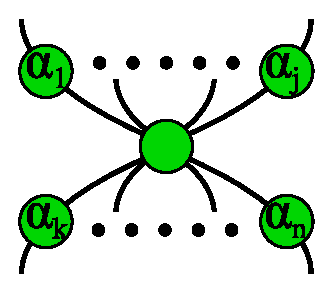
\includegraphics{images/spider_lhs.eps}}
\end{center}

\noindent Such pictures represent an infinite family of concrete
graphs. In this section we describe an extension of the representation
for Compact Closed Categories that allows a graph-based representation
that captures an infinite family of graphs. Notably, this allows us to
represent laws about quantum computation, such as
Spider-Law~\ref{spider-law-fig}. Furthermore, this representation is
still compositional in the sense that we can compose graphs. The
extension, which we call \ref{graph patterns}, adds two extra kinds of
nodes to the graph. Namely, {\em banged boxes} which informally
represent an arbitrary number of copies of a node (where the node is
defined as some graph), and {\em variable nodes} which informally
represent some, as yet unkown, node in a graph.

\subsection{Bang-Boxes}

Bang-Boxes 

\subsection{Variable Nodes}

In graph patterns, variable nodes generalise the concept of a
half-edge. A graph with variable nodes is given the following
interpretation in the underyling semantics of our concrete graphs:

Definition: super-type: given a node with type T

\begin{itemize}
\item let the node kinds be denoted by the set $K$
\item given a graph $G$ containing a set of variable nodes $V$ 
  a given node $n$, it's type is written $T_n$,
\end{itemize}

\subsection{Compositonality}

\subsection{Instantiation}


\section{Graph Pattern Rewriting}
\label{sec:rewriting}

\subsection{Rules}
\subsection{Unification}
\subsection{Substitution}


\section{Node Expressions}
\label{sec:node-expressions}


\section{Related Work}
\label{sec:relatedwork}

Initially one might be tempted to think that the usual notion of
subgraph might surfice for expressing matching, however it allows
additional edges on nodes where, because of the tensorial semantics of
our graphs, we do not. Our work provides a restriction of the usual
subgraph definition that is sound for Compact Closed Categories.

Link Graphs and their extention to BiGraphs also encapsualte a very
different kind of semantics where they allow edges to go to multiple
nodes. An interesting area of further work would be to consider our
graph patterns for these, and other, graph based formalisms.

Graph Grammars...

Other graph rewriting... 

Matrix Based Graph Tansformation...

Other Graph Transformation...

\section{Conclusions}
\label{sec:conclusions}

Ideas for further work
\begin{itemize}
\item simplification ordering
\item confluence arguments for graphs
\item formalise algorithms in a thm prover
\item richer graph structures - quantification over edges
\item richer expression language in vertices
\item completeness of rewrite rules with respect to wpHilb
\end{itemize}

\bibliographystyle{plain}
\bibliography{all}
\bibliography{bibfile}

\end{document}



